% compile with: pdflatex -shell-escape filename.tex
\documentclass[crop,svgnames,tikz,convert=pdf2svg]{standalone}
\usepackage{tikz}
\usetikzlibrary{positioning}

\newcommand\halfopen[2]{\ensuremath{[#1,#2)}}

\tikzset{box1/.style={draw, align=left, font=\tiny, minimum size=0.9cm}}
\tikzset{box2/.style={draw, align=left, font=\scriptsize, minimum height=0.9cm, minimum width=1.9cm}}
\tikzset{box3/.style={draw, minimum height=0.9cm, minimum width=3.9cm}}
\tikzset{box4/.style={draw, minimum height=0.9cm, minimum width=7.9cm}}
\tikzset{box5/.style={draw, minimum height=0.9cm, minimum width=15.9cm}}
\tikzset{label/.style={color=black!50, font=\tiny}}

\begin{document}
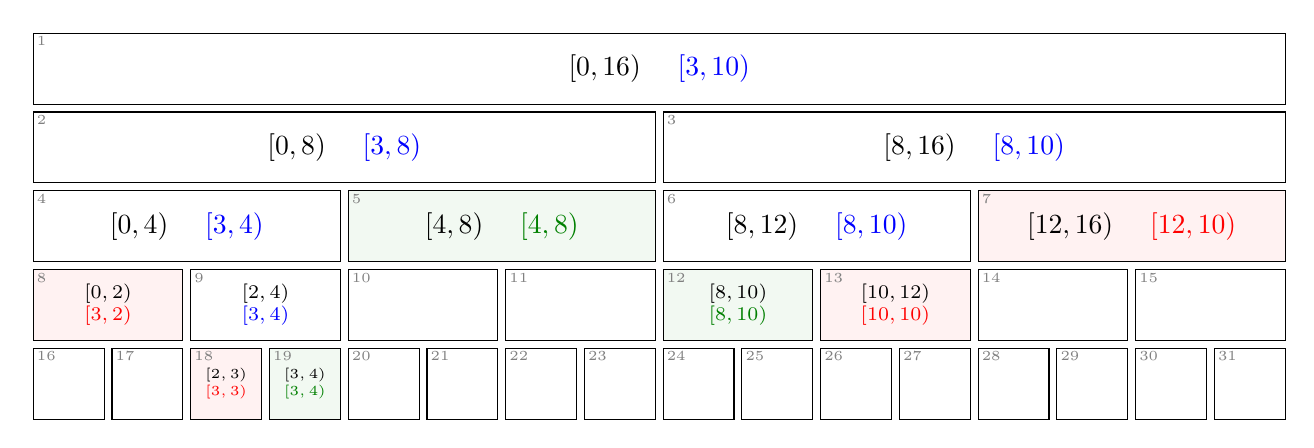
\begin{tikzpicture}

  \node [box5] at ( 7.5, 4) (node1)  {
    \halfopen{0}{16} \ \ \ {\color{blue} \halfopen{3}{10}}
  };

  \node [box4] at ( 3.5, 3) (node2)  {
    \halfopen{0}{8} \ \ \ {\color{blue} \halfopen{3}{8}}
  };
  \node [box4] at (11.5, 3) (node3)  {
    \halfopen{8}{16} \ \ \ {\color{blue} \halfopen{8}{10}}
  };

  \node [box3] at ( 1.5, 2) (node4)  {
    \halfopen{0}{4} \ \ \ {\color{blue} \halfopen{3}{4}}
  };
  \node [box3, fill=Green!5] at ( 5.5, 2) (node5)  {
    \halfopen{4}{8} \ \ \ {\color{Green} \halfopen{4}{8}}
  };
  \node [box3] at ( 9.5, 2) (node6)  {
    \halfopen{8}{12} \ \ \ {\color{blue} \halfopen{8}{10}}
  };
  \node [box3, fill=red!5] at (13.5, 2) (node7)  {
    \halfopen{12}{16} \ \ \ {\color{red} \halfopen{12}{10}}
  };

  \node [box2, fill=red!5] at ( 0.5, 1) (node8)  {
    \halfopen{0}{2}\\{\color{red} \halfopen{3}{2}}
  };
  \node [box2] at ( 2.5, 1) (node9)  {
    \halfopen{2}{4}\\{\color{blue} \halfopen{3}{4}}
  };
  \node [box2] at ( 4.5, 1) (node10) {};
  \node [box2] at ( 6.5, 1) (node11) {};
  \node [box2, fill=Green!5] at ( 8.5, 1) (node12) {
    \halfopen{8}{10}\\{\color{Green} \halfopen{8}{10}}
  };
  \node [box2, fill=red!5] at (10.5, 1) (node13) {
    \halfopen{10}{12}\\{\color{red} \halfopen{10}{10}}
  };
  \node [box2] at (12.5, 1) (node14) {};
  \node [box2] at (14.5, 1) (node15) {};

  \node [box1] at ( 0, 0) (node16) {};
  \node [box1] at ( 1, 0) (node17) {};
  \node [box1, fill=red!5] at ( 2, 0) (node18) {
    \halfopen{2}{3}\\{\color{red} \halfopen{3}{3}}
  };
  \node [box1, fill=Green!5] at ( 3, 0) (node19) {
    \halfopen{3}{4}\\{\color{Green} \halfopen{3}{4}}
  };
  \node [box1] at ( 4, 0) (node20) {};
  \node [box1] at ( 5, 0) (node21) {};
  \node [box1] at ( 6, 0) (node22) {};
  \node [box1] at ( 7, 0) (node23) {};
  \node [box1] at ( 8, 0) (node24) {};
  \node [box1] at ( 9, 0) (node25) {};
  \node [box1] at (10, 0) (node26) {};
  \node [box1] at (11, 0) (node27) {};
  \node [box1] at (12, 0) (node28) {};
  \node [box1] at (13, 0) (node29) {};
  \node [box1] at (14, 0) (node30) {};
  \node [box1] at (15, 0) (node31) {};

  \foreach \i in {1,...,31} {
%    \node [label, above left=-0.3 and -0.4 of node\i] {\i};
    \node [label, below right=-0.1 of node\i.north west] {\i};
  }

\end{tikzpicture}
\end{document}
